\newpage
\section{Auswertung}
\label{sec:auswertung}

Bei den folgenden Messauswertungen wurde ein Fehler von $\sqrt{N}$ bei $N$ gemessenen Ereignissen pro Kanal verrechnet, da diese Poisson verteilt sind.
Für alle \textit{fits}, die in der Auswertung vorkommen, wurde das \textit{python} Packet \textit{LMFIT} verwendet\cite{lmfit}.

\subsection{Halbwertsbreite bei variierender Verzögerung}
Es wurden für die Bestimmung der Halbwertsbreite, auch \enquote{full width at half maximum}, kurz fwhm, genannt, eine Verzögerung von je \SI{15}{\nano\second} bei beiden Verzögerungsleitungen eingestellt.
Daraus ergibt sich eine Verzögerungsdifferenz zwischen den beiden Leitungen zwischen -\SI{15}{\nano\second} und \SI{15}{\nano\second}.\\
Bei einem Messintervall von $\Delta t = \SI{10}{\second}$ werden die Pulse der PMTs gezählt und gegen die Verzögerungsdifferenz aufgetragen, was in \autoref{fig:fwhm} zu sehen ist.

\begin{figure}[H]
    \centering
    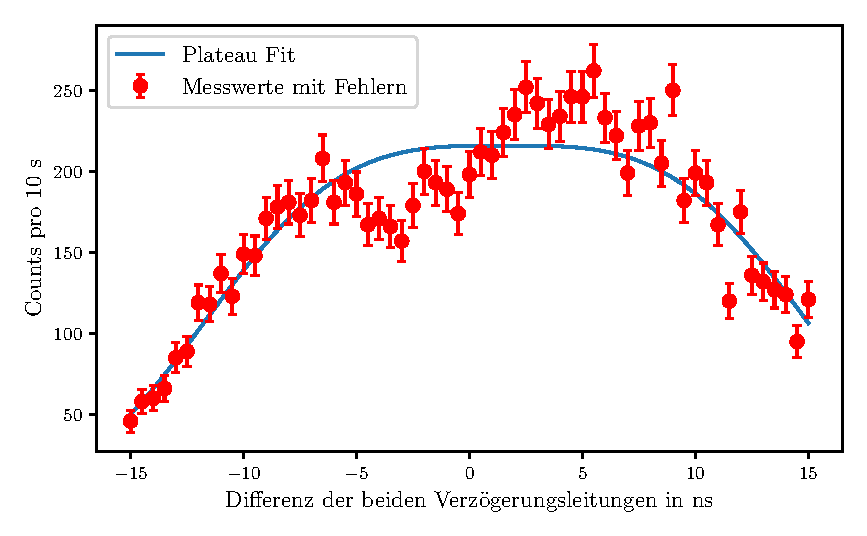
\includegraphics{images/fwhm.pdf}
    \caption{Gezählte Pulse bei verschiedenen Verzögerungseinstellungen der Verzögerungsleitungen, sowie ein Fit zur Annäherung des Verlaufs und zur Bestimmung des fwhm.}
    \label{fig:fwhm}
\end{figure}

Zur Bestimmung der Halbwertsbreite wurde der Verlauf der Messdaten an eine Gauss-Funktion angenähert.
Dies wurde lediglich genutzt, um die Halbwertsbreite auszurechnen, nicht weil die Messwerte tatsächlich einer Gauss-Funktion folgen.\\
In \autoref{fig:fwhm} ist dieser Gauss-Fit dargestellt, dessen Funktionsparameter berechnet wurden zu:
\begin{itemize}
    \item $A = 6546.1098 \pm 208.5633$
    \item $\mu = 2.4270 \pm 0.3405$
    \item $\sigma = 11.4103 \pm 0.4709$
\end{itemize}
bei einer Gauss-Funktion der Form
\begin{equation}
    f(x;A,\mu,\sigma) = \frac{A}{\sigma \sqrt{2\pi}}e^{\left[-\left(x - \mu\right)^2/{2\sigma^2}\right]}
\end{equation}.\\
Die Halbwertsbreite lässt sich aus dem Parameter $\sigma$ bestimmen über die Relation
\begin{equation}
    fwhm = 2\sqrt{2\ln2}\cdot \sigma
\end{equation}
und ergibt für diesen Gauss-Fit $fwhm = \left(26.8692\pm1.1089\right)\si{\nano\second}$.\\
Die Daten sind in \autoref{tab:fwhm} aufgelistet.

\subsection{MCA Kalibration}
\label{sec:calli}
Für die Kalibration wurden die Pulsabstände von \SI{0.3}{\micro\second} schrittweise um \SI{0.5}{\micro\second} erhöht bis \SI{9.8}{\micro\second}.
Diese Pulsabstände werden gegen den Index der Kanäle des MCA aufgetragen, was in \autoref{fig:linear} dargestellt ist.

\begin{figure}[H]
    \centering
    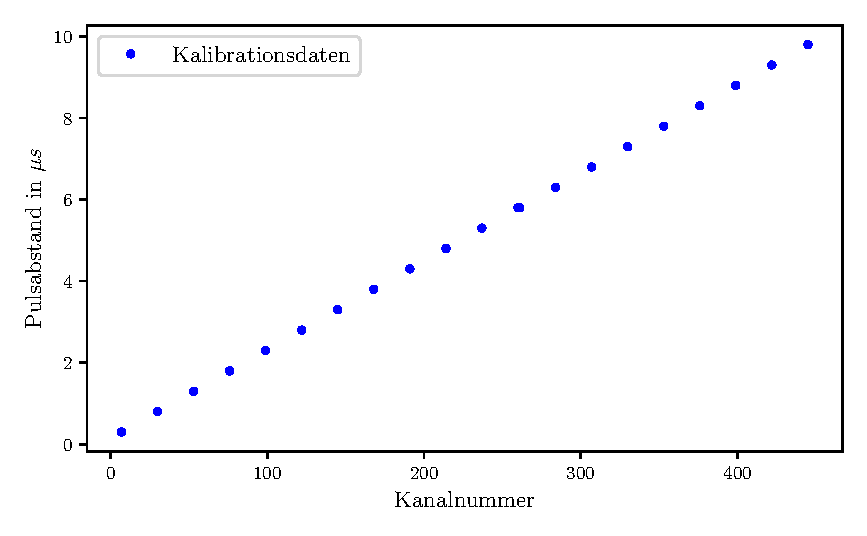
\includegraphics{images/linear.pdf}
    \caption{Abhängigkeit der Kanäle von dem Pulsabstand der Signale in \si[]{\micro\second}.}
    \label{fig:linear}
\end{figure}

Die Ausgleichsgerade ergibt eine Steigung von $0.0217\cfrac{\si{\micro\second}}{Kanal}$ und einen Startpunkt bei \SI{0.1542}{\micro\second}.
Die Funktion lautet somit
\begin{equation}
    f(x) = 0.0217x + 0.1542
\end{equation}
und gibt den jeweiligen Pulsabstand einer Kanalnummer an.\\
Die Daten sind in \autoref{tab:linear} aufgelistet.

\subsection{Berechnung der Untergrundrate}
Die Messung zeichnete 5635849 Start Signale auf und 15414 Stopp Signale.\\
Gemäß \autoref{eq:untergrund} wird zunächst der Erwartungswert der Verteilung $\lambda$ berechnet.
Die Suchzeit betrug $T_{Such} = $\SI{14}{\micro\second} und die totale Messzeit umfasste $t_{ges} = $\SI{253654}{\second}.
Daraus ergibt sich ein Erwartungswert von $\lambda \approx 311.06\cdot 10^{-6}$ und damit nach \autoref{eq:untergrund} ein Untergrund von $1752.55$.\\
Pro Kanal sind dies 3.423 Untergrundmessungen.

\subsection{Lebensdauer von Myonen}
In \autoref{fig:myonenroh} sind die rohen Messergebnisse nach ca. 3 Tagen totaler Messzeit in Abhängigkeit der Kanäle aufgetragen.

\begin{figure}[H]
    \centering
    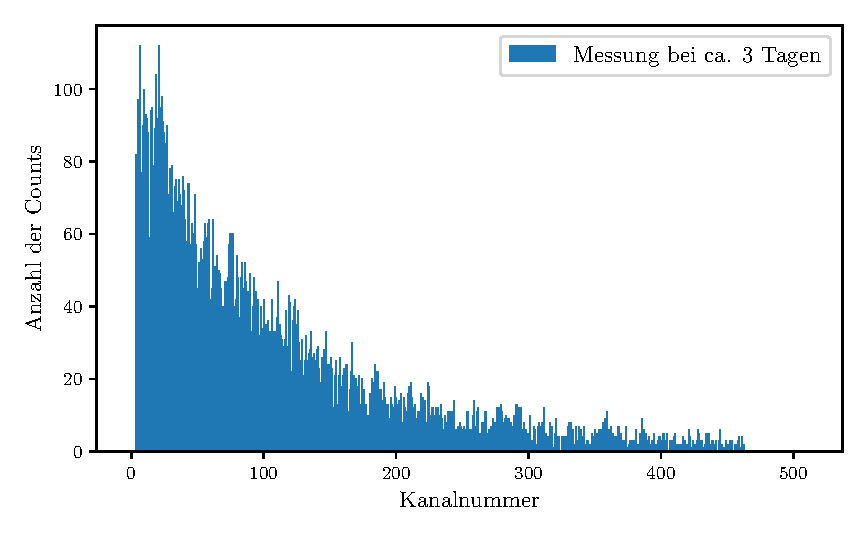
\includegraphics{images/messung_roh.pdf}
    \caption{Rohdaten nach ca. 3 Tagen Messung von Myonenlebensdauern.}
    \label{fig:myonenroh}
\end{figure}

Nach Konvertierung der Kanäle in Zerfallsdauern, mit der Ausgleichsgerade bestimmt in \autoref{sec:calli}, wird ein Fit an die Messdaten samt Unsicherheiten angelegt.
Das Ergebnis dieses Exponential-Funktion Fits, nach \autoref{eq:zerfall}, ist in \autoref{fig:myonen} dargestellt.

\begin{figure}[H]
    \centering
    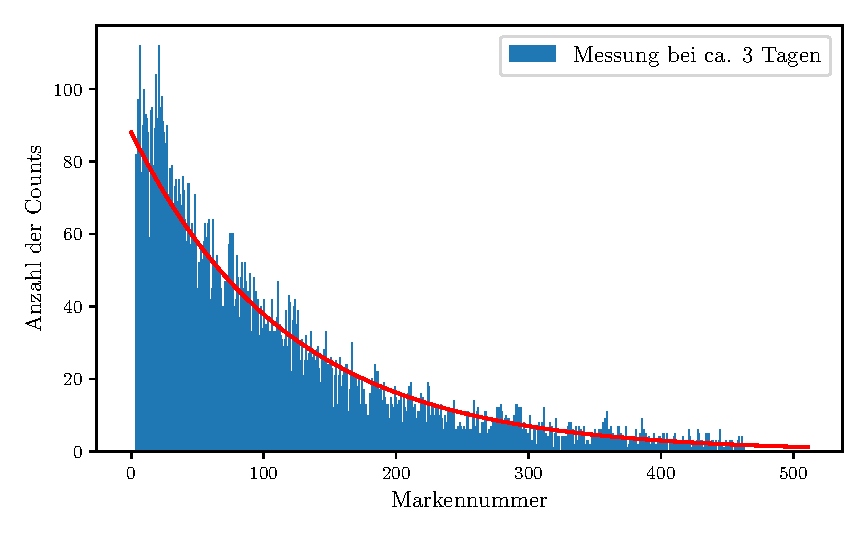
\includegraphics{images/messung_fit.pdf}
    \caption{Die Messdaten und der Fit der Messdaten samt Unsicherheiten sind gegen die Lebensdauer aufgetragen.}
    \label{fig:myonen}
\end{figure}

Die Fit-Parameter ergeben die Lebensdauer des Myons:
\begin{itemize}
    \item $N_0 = 93.6524 \pm 1.1433$
    \item $\tau = 2.5454 \pm 0.0417$\ \si{\micro\second}
\end{itemize}